\documentclass{standalone}
\usepackage{tikz}
\usepackage{xstring}
\begin{document}
	%no color

	\IfStrEq{\jobname}{\detokenize{graphnocolor}}{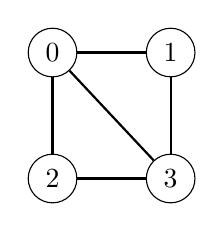
\begin{tikzpicture}
	\node[draw,circle,] (0) at (1,.8) {0};
	\node[draw,circle,] (1) at (2.5,.8) {1};
	\node[draw,circle,] (2) at (1,-.8) {2};
	\node[draw,circle,] (3) at (2.5,-.8) {3};
	
	\draw[thick] (0) -- (1) -- (3) -- (2) -- (0);
	\draw[thick] (0) -- (3);
	\end{tikzpicture}}{}


	\IfStrEq{\jobname}{\detokenize{graphcolor1}}{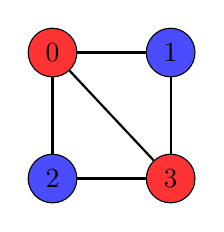
\begin{tikzpicture}
		\node[draw,circle,fill=red!80] (1) at (1,.8) {0};
		\node[draw,circle,fill=blue!70] (2) at (2.5,.8) {1};
		\node[draw,circle,fill=blue!70] (3) at (1,-.8) {2};
		\node[draw,circle,fill=red!80] (4) at (2.5,-.8) {3};
		
		\draw[thick] (1) -- (2)-- (4) -- (3) -- (1);
		\draw[thick] (1) -- (4);
		\end{tikzpicture}}{}

	\IfStrEq{\jobname}{\detokenize{graphcolor2}}{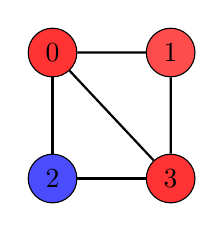
\begin{tikzpicture}
		\node[draw,circle,fill=red!80] (1) at (1,.8) {0};
		\node[draw,circle,fill=red!70] (2) at (2.5,.8) {1};
		\node[draw,circle,fill=blue!70] (3) at (1,-.8) {2};
		\node[draw,circle,fill=red!80] (4) at (2.5,-.8) {3};
		
		\draw[thick] (4) -- (3) -- (1);
		\draw[thick] (1) -- (4) -- (2) -- (1);
		\end{tikzpicture}}{}	

\IfStrEq{\jobname}{\detokenize{bipartite}}{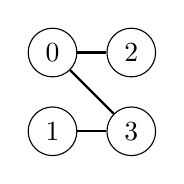
\begin{tikzpicture}
	\node[draw,circle] (a1) at (0,0) {0};
	\node[draw,circle] (a2) at (0,-1) {1};
	\node[draw,circle] (b1) at (1,0) {2};
	\node[draw,circle] (b2) at (1,-1) {3};
	
	\draw[thick] (a1) -- (b1);
	\draw[thick] (a1) -- (b2);
	\draw[thick] (a2) -- (b2);
	
	\end{tikzpicture}}{}

\IfStrEq{\jobname}{\detokenize{nonbipartite}}{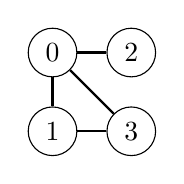
\begin{tikzpicture}
	\node[draw,circle] (a1) at (0,0) {0};
	\node[draw,circle] (a2) at (0,-1) {1};
	\node[draw,circle] (b1) at (1,0) {2};
	\node[draw,circle] (b2) at (1,-1) {3};
	
	\draw[thick] (a1) -- (b1);
	\draw[thick] (a1) -- (b2);
	\draw[thick] (a2) -- (b2);
	\draw[thick] (a1) -- (a2);
	
	\end{tikzpicture}}{}
	
\IfStrEq{\jobname}{\detokenize{path3}}{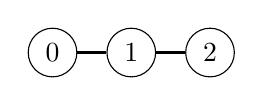
\begin{tikzpicture}
	\node[draw,circle] (0) at (0,0) {0};
	\node[draw,circle] (1) at (1,0) {1};
	\node[draw,circle] (2) at (2,0) {2};
	
	\draw[thick] (0) -- (1) -- (2);	
	\end{tikzpicture}}{}

\IfStrEq{\jobname}{\detokenize{completebipartite}}{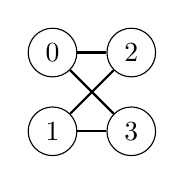
\begin{tikzpicture}
	\node[draw,circle] (a1) at (0,0) {0};
	\node[draw,circle] (a2) at (0,-1) {1};
	\node[draw,circle] (b1) at (1,0) {2};
	\node[draw,circle] (b2) at (1,-1) {3};

	\draw[thick] (a1) -- (b1);
	\draw[thick] (a1) -- (b2);
	\draw[thick] (a2) -- (b1);
	\draw[thick] (a2) -- (b2);
	\end{tikzpicture}}{}


\IfStrEq{\jobname}{\detokenize{finalgrover1}}{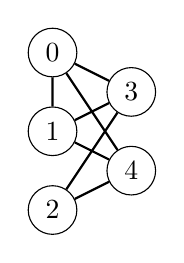
\begin{tikzpicture}
	\node[draw,circle] (0) at (0,0) {0};
	\node[draw,circle] (1) at (0,-1) {1};
	\node[draw,circle] (2) at (0,-2) {2};
	\node[draw,circle] (3) at (1,-.5) {3};
	\node[draw,circle] (4) at (1,-1.5) {4};

	\draw[thick] (0) -- (3) -- (1) -- (3) -- (2) -- (4) -- (0) -- (1) -- (4);
	\end{tikzpicture}}{}

	

\end{document}